% Timing of a dual-response task under the two reporting rules (@fig-timing).
% Rebuild both outputs from this directory with:
%   pdflatex timing.tex && pdftocairo -svg timing.pdf timing.svg
\documentclass[tikz,border=4pt]{standalone}
\usepackage{amsmath,amssymb}
\usetikzlibrary{arrows.meta,positioning,calc}

\begin{document}
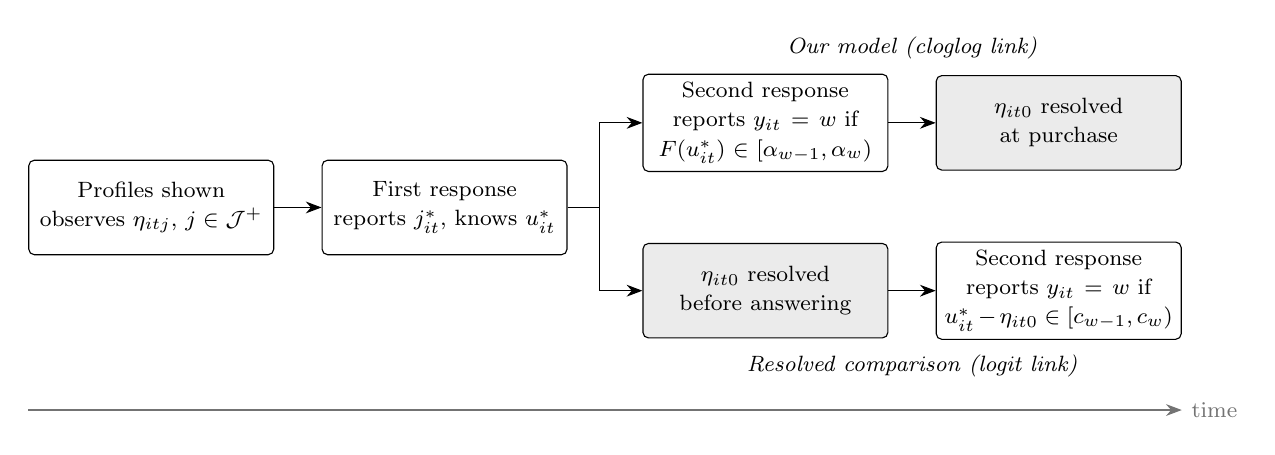
\begin{tikzpicture}[
  font=\footnotesize,
  >={Stealth[length=2mm]},
  stage/.style={draw, rounded corners=2pt, align=center, text width=2.9cm,
                minimum height=1.2cm, inner sep=3pt},
  resolve/.style={stage, fill=black!8},
  lane/.style={font=\footnotesize\itshape, align=center},
]

% Common trunk
\node[stage] (shown) {Profiles shown\\[1pt] observes $\eta_{itj}$, $j \in \mathcal{J}^{+}$};
\node[stage, right=0.6cm of shown] (choice) {First response\\[1pt] reports $j^*_{it}$, knows $u^*_{it}$};

% Our model: report first, outside good resolved later
\node[stage, above right=0.45cm and 0.95cm of choice.east, anchor=south west] (reportA)
  {Second response\\[1pt] reports $y_{it} = w$ if\\[1pt] $F(u^*_{it}) \in [\alpha_{w-1}, \alpha_w)$};
\node[resolve, right=0.6cm of reportA] (resolveA)
  {$\eta_{it0}$ resolved\\[1pt] at purchase};

% Resolved comparison: outside good resolved first, then report
\node[resolve, below right=0.45cm and 0.95cm of choice.east, anchor=north west] (resolveB)
  {$\eta_{it0}$ resolved\\[1pt] before answering};
\node[stage, right=0.6cm of resolveB] (reportB)
  {Second response\\[1pt] reports $y_{it} = w$ if\\[1pt] $u^*_{it} - \eta_{it0} \in [c_{w-1}, c_w)$};

\draw[->] (shown) -- (choice);
\draw[->] (choice.east) -- ++(0.4,0) |- (reportA.west);
\draw[->] (choice.east) -- ++(0.4,0) |- (resolveB.west);
\draw[->] (reportA) -- (resolveA);
\draw[->] (resolveB) -- (reportB);

% Lane labels: the reporting rule and the link it implies
\node[lane, above=2pt of $(reportA.north)!0.5!(resolveA.north)$]
  {Our model (cloglog link)};
\node[lane, below=2pt of $(resolveB.south)!0.5!(reportB.south)$] (laneB)
  {Resolved comparison (logit link)};

% Time axis
\coordinate (axisL) at ($(shown.west |- laneB.south) + (0,-0.3)$);
\coordinate (axisR) at ($(resolveA.east |- laneB.south) + (0,-0.3)$);
\draw[->, black!55] (axisL) -- (axisR) node[right, black!55] {time};

\end{tikzpicture}
\end{document}
